% vim: expandtab tabstop=2 softtabstop=2 shiftwidth=2
\documentclass[a4paper,12pt]{article}
%\usepackage[scale=.8]{geometry}
\usepackage[english,noconfigs]{babel}
\usepackage{ifluatex,ifxetex}
\ifnum 0\ifxetex 1\fi\ifluatex 1\fi=0 % if pdftex
  \usepackage[utf8]{inputenc}
  \usepackage[T1]{fontenc}
\fi

\usepackage[ruled]{algorithm2e}
\usepackage[toc,page]{appendix}
\usepackage{minted}

\usepackage{graphicx}
\graphicspath{{graphics/}}

\usepackage{lipsum}
\usepackage{hyperref}

\title{%
  \textbf{Universal predictor}\\\small%
  Pattern-based prediction algorithms,\\%
  applications \& variations%
}

\author{%
  Carolina de Senne Garcia\\%
  Clément Durand%
}

\begin{document}
\maketitle

\vspace*{\fill}

\begin{center}
  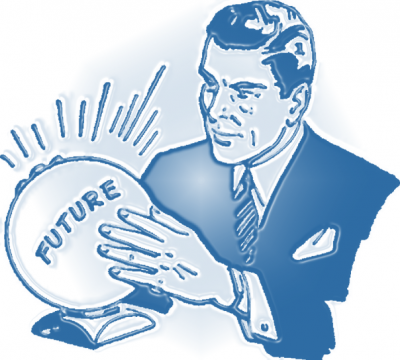
\includegraphics[width=0.6\textwidth]{images/future}
\end{center}

\vspace*{\fill}

\clearpage

\tableofcontents

\clearpage

\section*{Introduction}
\addcontentsline{toc}{section}{Introduction}

In this work we considered the problem of implementing an universal predictor based on patter matching. An universal predictor aims to perform well without knowing knowing the underlying probabilistic model of the data to be analysed.

In section \ref{paper_algos} we present an implementation of the basic idea of a predictor proposed by Ehrenfeucht and Mycielski \cite{basic_algo}, called \textit{Sampled Pattern Matching} (SPM) in \cite{paper}. Though the former was not an universal predictor, it was a good density estimator and was used by Jacquet et al. \cite{paper} as the base idea to develop an universal predictor. The implementation of this universal predictor is also presented in \ref{paper_algos}.

Section \ref{variation_algo} exposes a variation of the predictor algorithm proposed by us and based on Machine Learning techniques and pre-computation. We compare its performance with the universal predictor of section \ref{paper_algos}.

Finally, in section \ref{tests} we discuss performance tests for the algorithms implemented in this work, as well as implementation issues and possible solutions for them.

\section{Universal prediction algorithm}\label{paper_algos}

  In this section we present the algorithms from \cite{paper} which were implemented and tested in our work: the simplified version uses the longest suffix pattern match in the text we want to predict. The second version adds a parameter $\alpha$ to check for pattern matches of size $\alpha$ times the longest match size. The algorithms details are explained in their corresponding subsections bellow.

  \subsection{Simplified version}

  The base algorithm consists in finding the longest substrings from the input stream that match with the stream suffix (and that are not the suffix itself, of course). It then takes the most recent substring (in terms of the stream input data) from the set of longest substrings (which can be of size 1) and returns the character that follows this substring in the input data as a prediction. These steps are described in algorithm \ref{simplified}.

    % Explain the idea of the algorithm, and mention the algorithm

    \begin{algorithm}
      \KwData{Character flow \textit{input}.}
      \KwResult{Prediction \textit{output}.}

      \textit{patterns} \gets{}
        $\left\{ (\textit{substring},x) :%
        \textit{substring}\cdot x\subset\textit{input} \wedge
        \textit{input} = w\cdot\textit{substring} \right\}$
        with multiplicity\;

      \textit{maxlen} \gets{} $\max\{\#\textit{pattern} :
        (\textit{pattern},x)\in\textit{patterns}\}$\;

      \KwRet{$x$} where $(\textit{pattern},x)\in\textit{patterns}$ is the most
        recent pattern of length \textit{maxlen}\;

      \caption{\label{simplified}Simplified version of universal prediction.}
    \end{algorithm}

    The implementation for this algorithm is exposed in annex \ref{code_simplified}.

    % First implementation (annex A), non-optimized pattern search.

  \subsection{Adding refinements}

  The algorithm \ref{complete} introduced in \cite{paper} finds the longest suffix match, as previously. However, it includes a parameter $\alpha$ that is multiplied by the length of the longest suffix match found, giving a new length. We look at the suffix matches that have this new lenght and return the prediction character (the character following the match) with higher frequency among this set.

    \begin{algorithm}
      \KwData{Character flow \textit{input}, parameter $\alpha$.}
      \KwResult{Prediction \textit{output}.}

      \textit{patterns} \gets{}
        $\left\{ (\textit{substring},x) :%
        \textit{substring}\cdot x\subset\textit{input} \wedge
        \textit{input} = w\cdot\textit{substring} \right\}$
        with multiplicity\;

      \textit{len} \gets{} $\alpha\times\max\{\#\textit{pattern} :
        (\textit{pattern},x)\in\textit{patterns}\}$\;

      \KwRet{$x$} the most frequent among the patterns $(\textit{pattern},x)$
        of length \textit{len} in \textit{patterns}\;

      \caption{\label{complete}Universal prediction.}
    \end{algorithm}

    The implementation for this algorithm is exposed in annex \ref{code_complete}.

    \section{Variation proposal}\label{variation_algo}

    In certain contexts (e.g. languages) it could be useful to have an algorithm that learns from existing text  before performing a prediction. In this section we propose an algorithm that does so.
  
  \subsection{Learning algorithm}

  The learning algorithm consists in taking a string as input and producing the substring patterns tree from it, by limiting the maximum length of the substrings. This maximum length also corresponds to the height of the tree. The pseudocode is depicted in algorithm \ref{learning} and the implementation of it is displayed in annex \ref{code_learning}.

  \begin{algorithm}
    \KwData{Texts to read \textit{input}, memory size \textit{cache}.}
    \KwResult{Substrings and number of occurrences.}

    \textit{substrings} \gets{}
      $\left\{ \textit{substring} : \textit{substring}\subset\textit{input}
      \wedge \#\textit{substring} \leq \textit{cache} \right\}$
      with multiplicity\;

    \KwRet{\textit{substrings}} with multiplicity count\;

    \caption{\label{learning}Learning patterns by reading.}
  \end{algorithm}

  \subsection{Prediction algorithm}

  The prediction algorithm based on the construction of a substring tree consists in following directly the suffix path in the tree for the text we want to predict. The pseudocode is depicted in algorithm \ref{predicting} and the implementation of it is displayed in annex \ref{code_predicting}.

  \begin{algorithm}
    \KwData{Substrings and multiplicity counts.}
    \KwResult{Predictions}

    \KwRet{\textit{substrings}} with multiplicity count\;

    \caption{\label{predicting}Turning substrings into predictions}
  \end{algorithm}

  \subsection{Comparison}

  Althought the learning algorithm has a lower time complexity than the universal predictor (see section \ref{tests}), it is difficult to compare both algorithms, since the first has a very long precomputation time. This precomputation time, associated with the use of a big memory (the substring tree) enables the prediction part of the algorithm to have a very good performance.
  % Performance: difficilement comparable car on change l'équilibre du compromis
  % précomputation/prédiction.

  \section{Results, Analysis and issues}\label{tests}

  In this section we present theoretical results of the algorithms analysed and experimental results in terms of prediction precision for different values of the parameter $\alpha$ in the universal predictor. We also escribe the distributed method used to perform the predictions on parts of the Bible and on pseudorandom texts.

  \subsection{Performance Analysis}

  In terms of theoretical complexity, the implementation for the universal predictor proposed earlier has time complexity $O(n)$ for one prediction, hence $O(n^2)$ for the whole text (it takes, more precisely, $O(n^2/2)$). Its space complexity if $O(n)$, corresponding to the index set size.

  The variation algorithm has time complexity of $O(p)$, being $p$ the parameter determining the maximal height of the substring tree. In our case, we used $p=10$, so we have a time complexity of $O(10)$, hence constant $O(1)$. This huge improvement compared to the universal predictor is due to a pre-calculation to build the substring tree that takes much longer than the prediction algorithm and has a considerable space complexity.

  Concerning the universal predictor, we also wanted to study which values of $\alpha$ gave better prediction results. We display in Table \ref{alpha} the results of our tests.

 \begin{table}
    \centering
    \begin{tabular}{c || c  c}
      $\alpha$ & Lorem Ipsum & Bible \\\hline\hline
      1.0 & 58.97\% & 65.67\% \\\hline
      0.9 & 59.19\% & 65.30\% \\\hline
      0.8 & 59.26\% & 65.52\% \\\hline
      0.7 & 59.26\% & 65.30\% \\\hline
      0.6 & 57.58\% & 61.13\% \\\hline
      0.5 & 56.55\% & 64.10\% \\\hline
      0.4 & 51.78\% & 61.61\% \\\hline
      0.3 & 43.21\% & 57.21\% \\\hline
      0.2 & 34.90\% & 53.12\% \\\hline
      0.1 & 27.18\% & 44.82\%
    \end{tabular}
    \caption{\label{alpha} Precision performance for different $\alpha$ values applied to Lorem Ipsum and an extract from the Bible}
  \end{table}

  \subsection{Distributing the algorithms}

  For the universal predictor algorithm we implemented a distributed version in order to enhance its time performance. The main idea is to use several machines and divide the text to be predicted into chuncks that are analysed by each machine. Each machine then runs the original prediction over its piece of text and returns the statistics to a central computing server. The central server gathers the results received in order to merge them and produce the final prediction ratio.

  This idea was also applied to the learning algorithm, although it was not very interesting due to the merge time delays.
  
\section*{Lessons learned}
\addcontentsline{toc}{section}{Lessons learned}

\begin{center}
\url{https://youtu.be/k0XIBDZRwxw}
\end{center}

In this work we implemented algorithms that aimed to predict text based on previous text that was given. First of all we implemented a basic idea of prediction given by Ehrenfeucht and Mycielski \cite{basic_algo}. We also implemented the universal predictor proposed by Jacquet et al. \cite{paper} which was based in the basic idea and that took as a parameter $\alpha$, a real value between $0$ and $1$. We ran the universal prediction on human text (the Bible) and on pseudorandom text (Lorem Ipsum) for several values of $\alpha$: the results indicate that for human text, the most adapted value for $\alpha$ is $1$, while for pseudorandom text, it is between $\alpha=0.7$ and $\alpha=0.9$.

Finally, we proposed a variation algorithm for predicting text based on a precomputation learning algorithm: by constructing a substring tree for the input text, the calculation of a prediction inside this text is much faster. However, this low time complexity is balanced by the precomputation (that takes a long time) and by the extra memory space used to store the tree.

\bibliographystyle{plain}
\bibliography{references}

\clearpage
\begin{appendices}

  The algorithms presented in this report were implemented and evaluated
  in \emph{python3.5}. The code snippets below are simplified versions of
  the relevant parts of the implementation and are not $100\%$ correct for
  simplicity sake. Comments were added for clarity and the full source code
  remains available.

  \section{Simplified universal prediction}\label{code_simplified}

    \inputminted[linenos]{python}{code/simplified.py}

  \clearpage
  \section{Universal prediction}\label{code_complete}

    \inputminted[linenos]{python}{code/complete.py}

  \clearpage
  \section{Learning and predicting}

  \subsection{Learning algorithm}\label{code_learning}

      \inputminted[linenos]{python}{code/learning.py}

    \clearpage
    \subsection{From substrings to predictions}\label{code_predicting}

      \inputminted[linenos]{python}{code/predicting.py}

\end{appendices}

\end{document}
